%!TEX root = ../../main.tex
\chapter{関連研究}
\section{動作・開発環境}
本研究の動作・開発環境について述べる.

\subsection{Intel RealSense 3D Camera}
旋律線とリズムの直感的な入力手段として使用した.RealSenseは手指やジェスチャー,顔の部位や表情,心拍や音声,対象物の奥行きなどを認識することができる.さらに,今後各国の主要PCメーカーがRealSenseを内蔵したPCを発売することに賛同している.従来,Kinect\footnote{http://www.xbox.com/ja-JP/kinect}をはじめとするモーションセンサ類を使用するにはわざわざデバイスを購入しなければならず,モーションセンサ類の存在を知らなかったり,存在を知っていても新たにデバイスを用意する手間や安価であっても購入の費用を嫌う人は一部のユーザーが使うものという認識であった.RealSense搭載PCの増加やWindows Helloなどモーションセンサでの開発経験のない一般ユーザーでも,容易に手に入ったり認知することができるRealSenseはその普及度においても期待されているデバイスである.

\subsection{Processing}
本システムの実装には,RealSense SDKを扱うことができ,画像や音声を比較的容易に行うことができるプログラミング言語Processingを用いる.Processing\footnote{https://www.processing.org/}は,MIT(Massachusetts Institute of Technology)メディアラボに所属していたCasey ReasとBen Fryによって開発された,視覚芸術のためのプログラミング教育ように作られたJavaをベースにした開発環境である.\cite{takahasi2010}
\section{関連研究}
本研究と関連のある研究やシステムを紹介する.

\subsection{Songle}
Songle\cite{songle}とは,音楽をサビ,メロディ,コード,ビートなどの構造を表示しながら鑑賞できるサービスで,ピアプロ\footnote{http://piapro.jp/}やSoundCloud\footnote{https://soundcloud.com/}の楽曲ページ,ニコニコ動画\footnote{http://www.nicovideo.jp/}やYouTube\footnote{https://www.youtube.com/}などにアップロードされている合法的に視聴可能な楽曲を音楽理解技術により自動解析しAメロ・Bメロ・サビといった繰り返し構造や、ビートの位置・コード進行・ボーカルの音高などを自動的に解析して見ることができる.さらにSongle上では複数のユーザでコンピュータの自動解析による誤差を訂正することで,解析結果の精度を高めている.また,Songle解析結果をJavaScriptから操作し,WEB上で利用するためのSongle Widget API\footnote{https://widget.songle.jp/}を用いることによって解析結果をJSONファイルとして参照することができる.

\subsection{KAGURA}
中村ら\cite{nakamura2010}はRealSenseを利用した音楽演奏アプリKAGURA\cite{kagura}を開発した.KAGURAはRealSenseを使用することによりRealSenseの特徴であるジェスチャー認識機能を利用し,身体動作で音の高さを,ジェスチャーで細かい設定や操作を指定することができる.出力される音は不協和音にならないようになっているため,適当に体を動かしたり,音楽演奏経験のない人でも音楽を演奏することができる.
また,KAGURAには録画機能とYouTubeへのアップロード機能が付いているため,気に入った演奏をすぐにインターネット上に公開することも容易に行えるようになっている.
\subsection{Airstic Drum}
菅家ら\cite{kanke2013}は,物理的に打面のあるドラム楽器(以下,実ドラム)の問題点を解決するために,実ドラムの補助として使用頻度の少ない打楽器に対して仮想ドラムを適用することで実ドラムと仮想ドラムの両方の利点を持ったAirstic Drumを設計した.この仮想ドラムの実装は無線通信機能を持つ加速度センサを搭載したドラムスティックから得られる加速度,角速度に閾値を設定し音の出力タイミングとしている.具体的には,加速度が設定された閾値(以下,基準強度)を超え,再び基準強度を下回るまでの経過時間の実ドラムと仮想ドラムの違いを識別して仮想ドラムの叩打タイミングとしている.また,仮想ドラムの叩打と演奏音の出力タイミングの時間差を測定するため,60bpm,90bpm,120bpmのテンポでメトロノームに合わせて仮想ドラムの叩打を繰り返し,メトロノームのクリック音とMIDI音源にメッセージが送信されるタイミングの時間差を計測した.

\subsection{調性理解モデルPFG Tonnetz}
白松ら\cite{shiramatsu2015}は調性理解モデルPFG Tonnetz (Prime Factor-based Generalized Tonnetz)を考案した.ある調の主音の周波数と協和音程の周波数比は,

\begin{align}
f=\Bigl(\prod_{pはn以下の素数} p^{(z_p)}\Bigr)\cdot f_{\rm tonic} ~~(z_pは整数)
\end{align}

のような素数の積で表すことができる.白松らは$n=5$と置いた上で,オクターブ隔たった音は音楽的に等価であることを考慮し,2の指数$z_2$軸をなくして$z_{3}z_{5}$平面へ投影すると,

\begin{figure}[t]
\begin{center}
	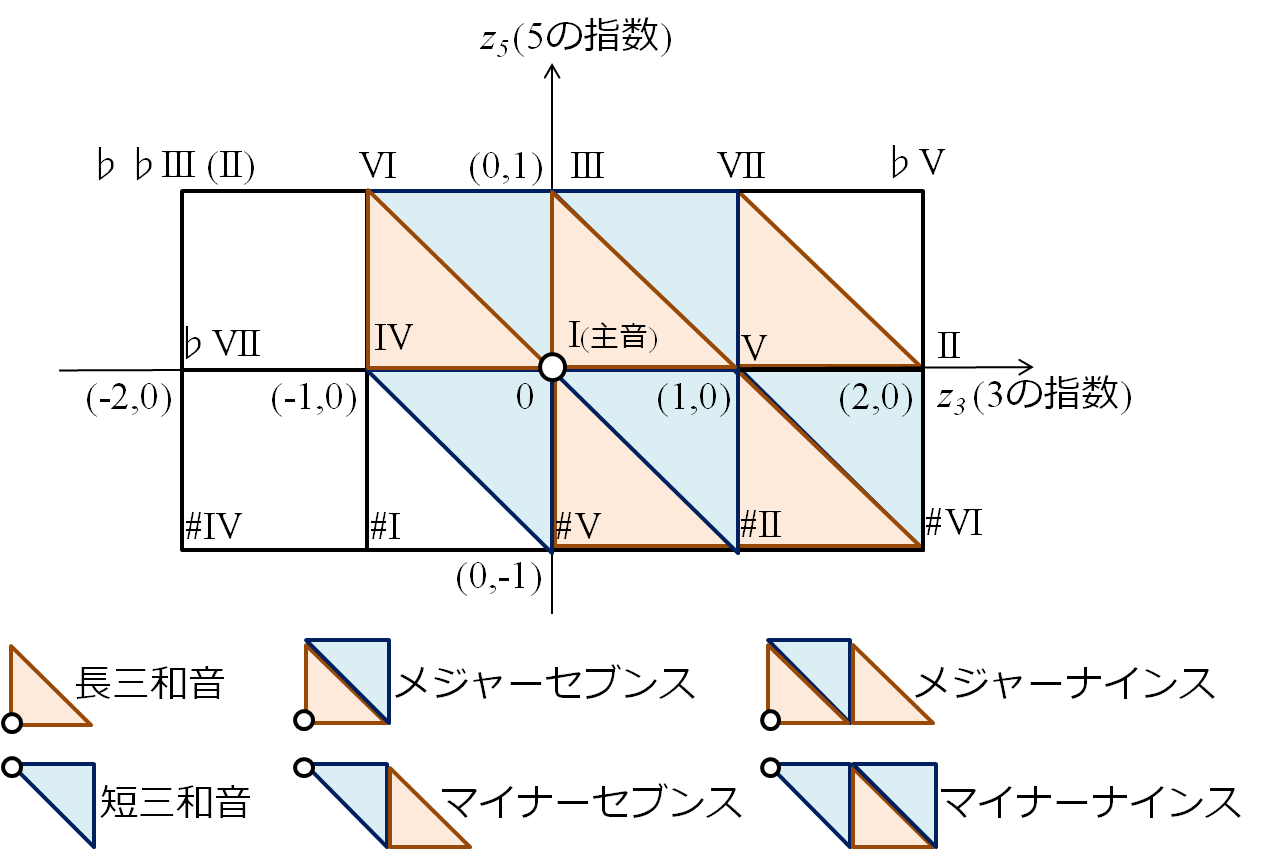
\includegraphics[width=0.9\linewidth]{assets/img/pfg-tonnetz.png}
	\caption{調性理解モデル PFG Tonnetz (5-limit)\cite{shiramatsu2015}}
	\label{img:pfg-tonnetz}
\end{center}
\end{figure}
図\ref{img:pfg-tonnetz}のように$z_3z_5$平面に配置される.この平面上の根音$(a,b)$に対して以下のような整数格子点列$\mathrm{chord}(a,b,\delta,m)$を考える.

\begin{align}
\mathrm{chord}(a,b,\delta,m)=\bigl[(a,b)+\sum_{i=0}^k \delta(i)\bigr]_{k=0,1,\cdots,m} \label{eq:code}\\
\delta_{\rm maj}(i)=\begin{cases}(0,1)&(iが奇数のとき)\\(1,-1)&(iが偶数のとき)\end{cases} \label{eq:maj}\\
\delta_{\rm min}(i)=\begin{cases}(1,-1)&(iが奇数のとき)\\(0,1)&(iが偶数のとき) \label{eq:min}\end{cases}
\end{align}

根音$(a,b)$を調の主音$(0,0)$で置き換えて考えると,明るい長音階の構成音(I, II, III, IV, V, VI, VII)が原点の上側$0 \leq z_5 \leq 1$に分布し,暗い短音階の構成音(I, II, \#II, IV, V, \#V, \#VI)が原点の下側$-1 \leq z_5 \leq 0$に分布するのが見て取れる.

このモデルは,音名,階名,コード名のようなシンボルを前提としては用いておらず,周波数比に基づく認知的原理のみから導かれる.まとめると,導出の過程で現れた以下の表現形式は,上記の認知的原理および導出されたモデルの観察から自然に導かれたものである.

\begin{itemize}
\item 整数格子点$(z_3, z_5)$: 音階の構成音,階名
\item 三角形$\bigl[(a,b)$, $(a,b+1)$, $(a+1,b)\bigr]$:\\
~~~ 整数格子点$(a,b)$を根音とする長三和音
\item 三角形$\bigl[(a,b)$, $(a+1,b-1)$, $(a+1,b)\bigr]$:\\
~~~ $(a,b)$を根音とする短三和音
\item 整数格子点列$\mathrm{chord}(a,b,\delta_{\rm maj},m)$:\\
~~~ $(a,b)$を根音とする長和音
\item 整数格子点列$\mathrm{chord}(a,b,\delta_{\rm min},m)$:\\
~~~ $(a,b)$を根音とする短和音
\end{itemize}

このPFG Tonnetzは数学者Leonhard Eulerが1739年に考案した調性理解モデルをもとに.
音楽学者Hugo Riemannが1880年に発展させたTonnetzというモデルに似ている
Tonnetzは1980年代以降,数学的に定式化された新リーマン理論(NeoRiemannian theory)へと発展し,様々な拡張が行われた\cite{behringer10}%\cite{tymoczko12}
が基本的には図\ref{img:euler},図\ref{img:riemann}のように音名同士を繋いだモデルであり,調の主音は表現できていない.
\begin{figure}[t]
	\begin{center}
		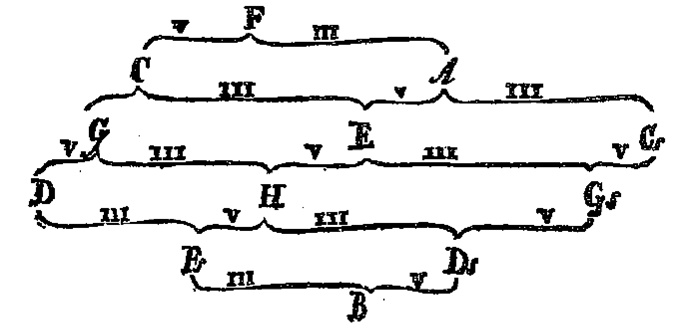
\includegraphics[width=0.9\linewidth]{assets/img/Eulers_tonnetz.png}
		\caption{Eulerの調性理解モデル\cite{shiramatsu2015}}
		\label{img:euler}
	\end{center}
\end{figure}
\begin{figure}[t]
	\begin{center}
		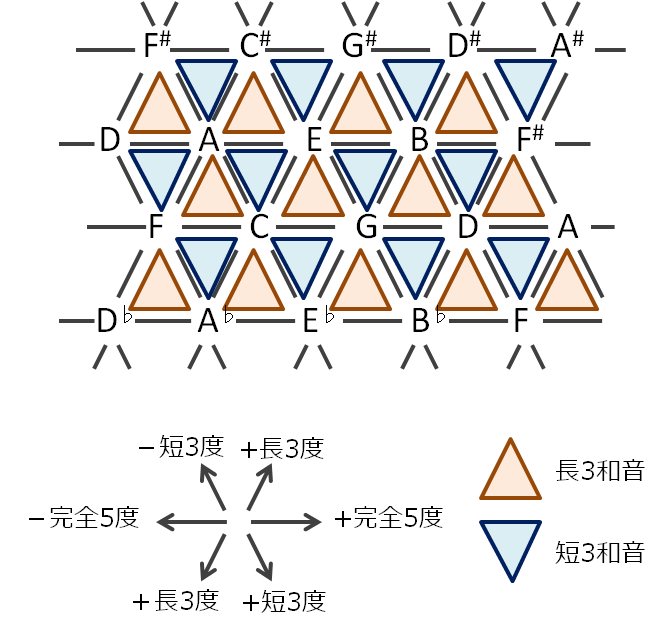
\includegraphics[width=0.9\linewidth]{assets/img/tonnetz_vertical.png}
		\caption{Riemannの調性理解モデル\cite{shiramatsu2015}}
		\label{img:riemann}
	\end{center}
\end{figure}
